%
% $Id: thesis_sample.tex 913 2017-12-22 09:21:50Z fukuyasu $
%
\documentclass[11pt]{jreport}
\usepackage{wuse_thesis}
\usepackage{indentfirst}
\usepackage{amsmath}
\usepackage{amssymb}
%\usepackage{url}	% \url{}コマンド用．URLを表示する際に便利
%\usepackage{graphicx}  % ←graphicx.styを用いてEPSを取り込む場合有効にする
			% 他のパッケージ・スタイルを使う場合には適宜追加
\usepackage[dvipdfmx]{graphicx}
%%%%%%%%%%%%%%%%%%%%%%%%%%%%%%%%%%%%%%%%%%%%%%%%%%%%%%%%%%%%%%%%%%%%%%%%

%%
%% 主に表紙を作成するための情報
%%

%%  タイトル(修論の場合は英語表記も指定)
\title{アニメにおける雲をCGで表現する方法の開発}
%\etitle{Test\\Test\\Test}

%%  著者名(修論の場合は英語表記も指定)
\author{坂口 美優}
%\eauthor{Naoki Fukuyasu}

%% 卒業論文・修士論文(以下のどちらかを選択)
\bachelar	% 卒業論文(4年生用)
%\master  	% 修士論文(M2用)

%%  学科・クラスタ
%\department{情報通信システム}
\department{デザイン情報}
%\department{デザイン科学}

%%  学生番号
\studentid{60195023}

%%  卒業年度
\gyear{2018}		% 提出年が2018年なら，2017年度

%%  論文提出日
\date{2018年2月14日}	% 修士の場合は月(2016年2月)までとし，英語表記も指定
%\edate{February 2018}	% 修士の場合，こちら(英語表記)も有効化

%%%%%%%%%%%%%%%%%%%%%%%%%%%%%%%%%%%%%%%%%%%%%%%%%%%%%%%%%%%%%%%%%%%%%%%%

\begin{document}

\maketitle

%%
%%  概要
%%
\begin{abstract}
　現在，映画やCMなどさまざまな映像において，水などの液体や炎，煙などのCGシミュレーションはあらゆる場面で多く使用されている．なかでも液体の表現は，物理現象に従う現実のものと見分けがつかないほどリアルなものから，性質(見た目)は液体で，物理現象に従わない実際にはありえない表現まで幅広く表現されている．このような表現は炎や煙のでも幅広く表現されている．しかし，雲の場合，物理現象に従う非常にリアルな表現方法は多く研究されているが，雲の性質を持ち物理現象に従わないものの表現，アニメで表現されているような雲の性質を持つが，実際の雲ではありえない触れたり乗れたりするような表現方法の研究ははとんど行われていない．\\
　本稿ではこのアニメで表現されている触れる，乗れるといった挙動をする雲をCGで表現する方法の開発を行う．現実にある雲を表現するのではなく，インタラクティブ性を考慮し，物体が本研究で開発する雲のようなものに当たると，実際の雲のように突き抜けるのではなく，触れる，形が変わるといった様子を表現する．提案の手法として，雲のようなものの見た目は実際の雲と同じように半透明の粒子を使い表現する．雲のようなものの挙動は，ばねの物理法則を用い，粒子間の力を計算し表現する．ある一定以上の力が加わると千切れる表も表現も行う．\\



\end{abstract}

%%  目次
\tableofcontents

%%  図目次 (図目次をいれたければ以下のコメントをはずす)
%\listoffigures

%%  表目次 (表目次をいれたければ以下のコメントをはずす)
%\listoftables

\newpage
\pagenumbering{arabic}	% 以降のページ番号を算用数字に

%%%%%%%%%%%%%%%%%%%%%%%%%%%%%%%%%%%%%%%%%%%%%%%%%%%%%%%%%%%%%%%%%%%%%%%%

%%
%%  本文はここから
%%
　

\chapter{第1章 はじめに}
　(参考文献　谷川さんの)
　現在，映画やCMなどの映像，ゲームや映画などにおいて，CGが使われていない映像は無いといっても過言ではないほどあらゆる場面でCGが使われている．その中でも流体に分類される雲や煙，水，はちみつのシミュレーションモデルとなる粘性体，炎などは特に多く表現されており，現実のものと見分けがつかないほどリアルな表現が可能となっている．流体の表現には物理現象に従ったリアルなものから流体の性質（見た目）をもった物理現象に従わないものなど幅広く表現されている．[図\ref{fig:fluidreal1} 図\ref{fig:fluidreal2}]本稿では流体のなかでも雲に重点おく．雲の表現はほかの流体とは異なり，主に物理現象に従ったリアルなものの表現手法が多く研究されている．[図\ref{fig:cloudreal}]一方，アニメで表現されているような触ることが出来たり，乗ることが出来るような雲はあまり表現されていない．本研究は，この乗る，触るといったアニメで表現されている，雲の性質を持つが物理現象に従わない雲のようなものをCGで表現する方法の開発を行う．\\
　アニメでは上記のように雲に乗ることが出来，触ることが出来る表現がある．[図\ref{fig:cloudanime}]また，一定以上の力が加わると散り散りになるという表現も行われている．しかし，現実にある雲は，空気中の水蒸気やちりが上昇気流によって上空に上がり，これが気圧の低下に伴い空気が膨張することによって温度が下がっている上空で冷やされる．すると，それまで見えない形で存在していた空気中の水蒸気が空気中のちりの周りに集まり，水滴や氷の結晶となって現れる．[図\ref{fig:howtobecloud1} 図\ref{fig:howtobecloud2} 図\ref{fig:howtobecloud3} 図\ref{fig:howtobecloud4}]これらが集まって出来ているのが雲なので触ることはできない．このように実際には触れない雲をアニメで表現されているような触れる雲の性質をもった雲ではない物質をCGでリアルに表現する方法を開発する．\\
　CGで雲のシミュレーションを行う方法は，実際にある雲のリアルな表現方法の開発やシミュレーションする方法はStamが開発した流体力学のNavierStokes方程式を用いた方法やNagelらによるセラルオートマンを使用した方法，菊池らによるパーティクルを利用した方法など様々な形で研究されているが，実際の雲と異なり，本研究で扱うのは触れる，乗れるような雲の性質をもった実際の雲ではないものの表現なので，これらの研究とは別の表現方法を用いる．\\
　本研究では，物体が触れると触れる，乗れるといった形が変わる部分の表現をばねの物理的挙動を用いて，粒子間につながりを持たせることで表現する．この時の弾性力は0とするので跳ね返る表現は行わない．また，一定以上の力が加わると散り散りになる表現は，ばねに一定以上の力が加わると途切れる物理法則を用いる．\\

\begin{figure} [htbp]
\begin{minipage}{0.5\hsize}
  \begin{center}
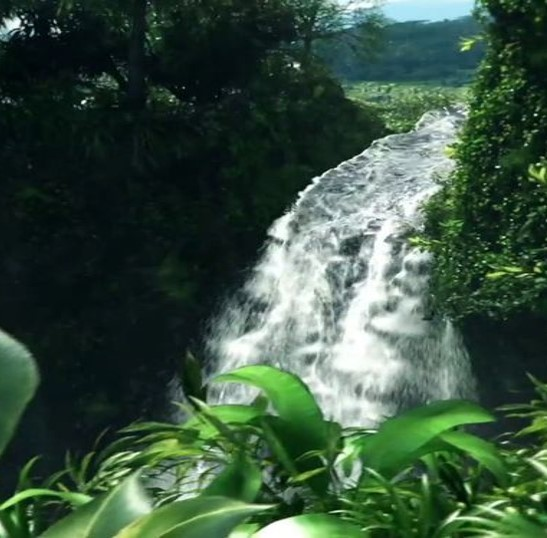
\includegraphics[height=5cm]{cgliquid1.jpg}
  \end{center}
  \caption{液体物理法則にしたがうリアルな表現}
  \label{fig:fluidreal1}
 \end{minipage}
\begin{minipage}{0.5\hsize}
  \begin{center}
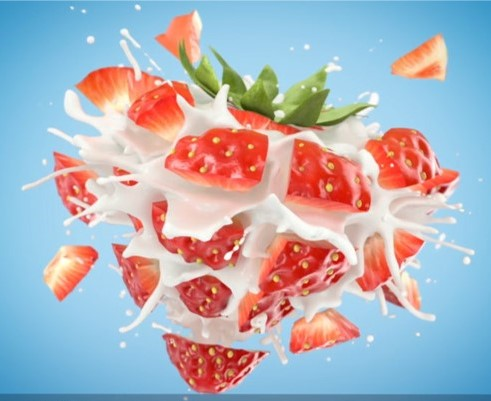
\includegraphics[height=5cm]{cgliquid3.jpg}
  \end{center}
  \caption{物理法則に従わない液体の表現}
  \label{fig:fluidreal2}
 \end{minipage}
\end{figure}

\begin{figure} [htbp]
  \begin{center}
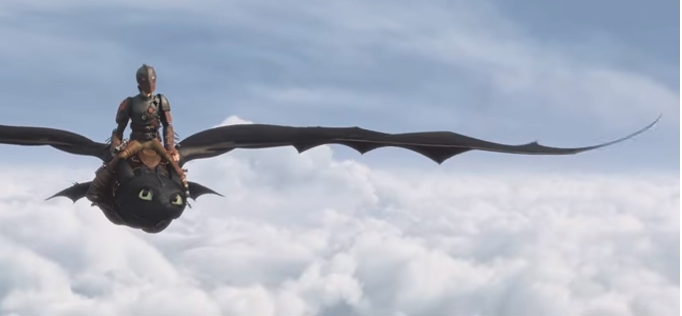
\includegraphics[width=10cm]{cgcloud1.png}
  \end{center}
  \caption{背景で用いられるリアルな雲の表現}
  \label{fig:cloudanime}
\end{figure}
\begin{figure} [htbp]
  \begin{center}
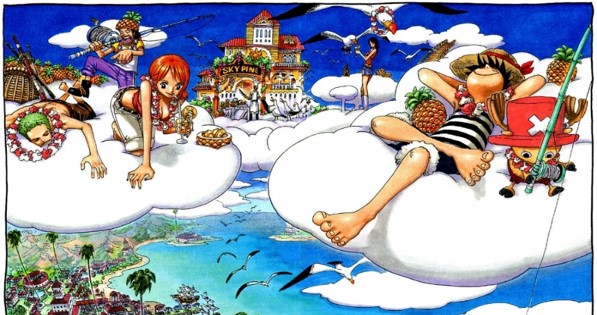
\includegraphics[width=10cm]{transformcloud1.jpg}
  \end{center}
  \caption{アニメで用いられる雲の表現}
  \label{fig:cloudanime}
\end{figure}


\begin{figure} [htbp]
\begin{minipage}{0.5\hsize}
  \begin{center}
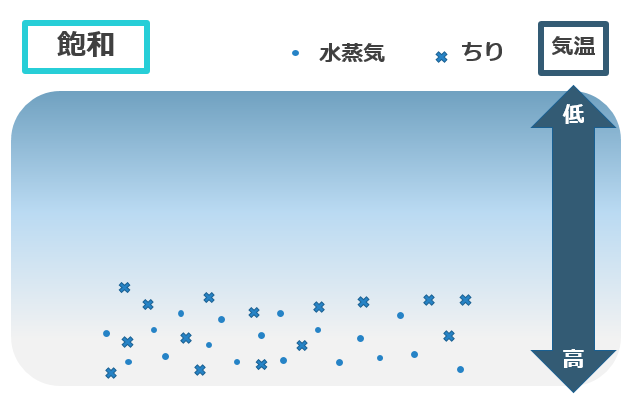
\includegraphics[height=5cm]{howtobecloud1.PNG}
  \end{center}
  \caption{背景で用いられるリアルな雲の表現}
  \label{fig:howtobecloud1}
 \end{minipage}
\begin{minipage}{0.5\hsize}
  \begin{center}
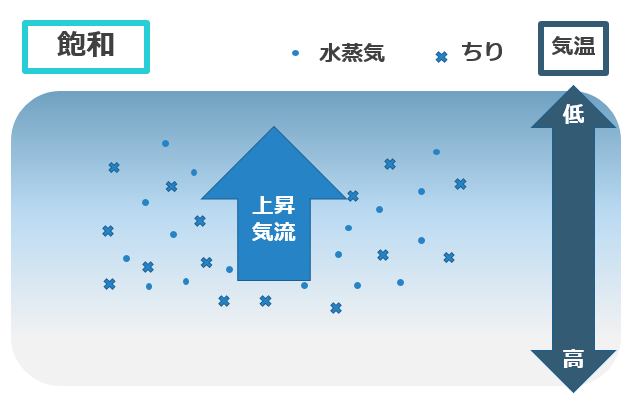
\includegraphics[height=5cm]{howtobecloud2.PNG}
  \end{center}
  \caption{アニメで用いられる雲の表現}
  \label{fig:howtobecloud2}
 \end{minipage}
\end{figure}
\begin{figure} [htbp]
\begin{minipage}{0.5\hsize}
  \begin{center}
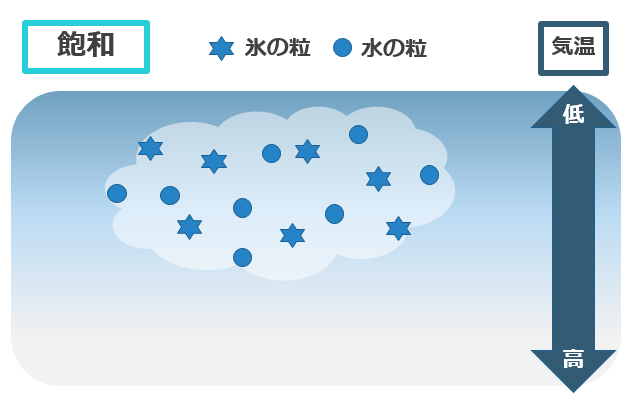
\includegraphics[height=5cm]{howtobecloud3.PNG}
  \end{center}
  \caption{背景で用いられるリアルな雲の表現}
  \label{fig:howtobecloud3}
 \end{minipage}
\begin{minipage}{0.5\hsize}
  \begin{center}
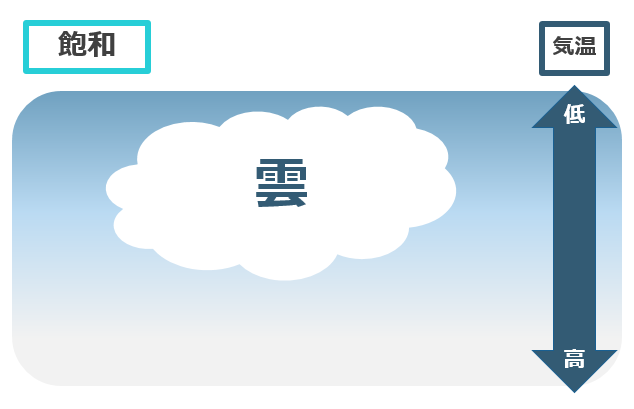
\includegraphics[height=5cm]{howtobecloud4.PNG}
  \end{center}
  \caption{アニメで用いられる雲の表現}
  \label{fig:howtobecloud4}
 \end{minipage}
\end{figure}


\chapter{提案手法}
本研究で開発する，雲のようなものの形と挙動について手法を提案する．

\section{モデリング}
　モデリングとは，CGによる画像生成においてまず描画したい物体の形や色，位置，大きさなどをコンピュータ内部で表現するために，物体の形状をデータ化することを言う．ここでは本研究で作成する雲のような物体をより雲らしい見た目にするための手法を提案する．

\subsection{パーティクル}
(3次元CGの基礎と応用[新訂版]千葉則茂・土井章男共著p12)
　CGの分野では流体は粒子(パーティクル)の集合体で表現されることが多い．火花や水滴はもちろん，炎，雲，霧などのガス状物体はパーティクル(粒子)の集合で表すことが出来る．たとえば，火花はパーティクルに初期速度，初期の形や色，生成時期，移動方法，生存期間などをあらかじめ定めておき，ある時点で生成されているパーティクルを表示することにより表現することが出来る．このようにモデリングがシミュレーション(アニメーション)と密接に関連する自然現象の表現にはパーティクルにより表現が適している．このことから、本研究においても見た目はパーティクルを用いて表現する．

\section{形の形成}
　本研究では見た目は雲のように見えるものを形成する必要がある．ここではその手法について提案する．本研究では，以下の図のような形をする[図\ref{fig:cloud}]4つの円の塊が集まってできたような形を形成することにする．円の塊を発生させるために，まず初めにそれぞれの円の中心となる粒子を発生させる．次にその中心部分の粒子から一定の範囲にランダムで円形に粒子を発生させ円形の粒子群を作成する．この円形の粒子群の位置はメルセンヌツイスター法を用いてすべての値の出現確率が等しい乱数である一様乱数によって決め，それぞれの中心から正規分布を用いて一定の範囲内に粒子を円形に発生させる．この方法を以下で詳しく説明していく．
\begin{figure} [htbp]
  \begin{center}

\includegraphics[width=5cm]{cloud.jpg}
  \end{center}
  \caption{本研究で作成する雲の形}
  \label{fig:cloud}
\end{figure}

\subsection{メルセンヌツイスター法}
(論文Mersenne Twister(松本・西村[1998]))
(参考サイト　統計数理研究所　疑似乱数発生法　メルセンヌツイスタ)
乱数生成の方法には線形合同法やM系列，メルセンヌツイスター法などがある．線形合同法は本来C言語の標準ライブラリの乱数生成器rand()では「線形合同法」というアルゴリズムが採用されていた．この方法は高速だが，周期が短いため大量の乱数列を使用するシミュレーションでは用いることが出来ない．また，下位ビットのランダム性が低いことや多次元で均等分布しない性質がある．M系列は線形合同法を改良したものではあるが，最大周期がにとどまりこれも大量の乱数列を使用するシミュレーションでは十分ではない．これに加えて出力されたすべてのビットが統計的に十分ランダムではないことと初期値の値についていい選択をしないと質の悪い乱数が生成されてしまう．
これらに対して，M系列を松本眞と西村拓士が発展させたメルセンヌツイスター法は，最大周期が証明されており，また高次元に均等に分布し，連続で出力された乱数列間に相関が無いものとして乱数列を扱うことができる．さらに出力されたすべてのビットが統計的に十分ランダムである．以上から本研究ではメルセンヌツイスター法を使用して乱数を生成している．

\subsection{正規分布}
(入門統計学橋本智雄著p61)
　偶然的事象を説明する数学的モデルとして，統計学では確率関数p(x)や密度関数f(x)をあらかじめ定めた確率モデルを仮定する．各種の統計現象においてしばしば登場してくるいくつかの主要な確率分布のなかに正規分布がある．本研究ではこの正規分布を用いて粒子を一定範囲内に発生させる．
　正規分布とは密度関数f(x)がすべてのxに対して(式)
で与えられるとき，Xの分布を正規分布といい，N(\mu，\sigma^{2})で表す．
　ここで，\mu，\sigma^{2}は定数(パラメータ)で\sigma>0である．このf(x)が密度関数になるのは，(式)
から確かめられる．(もっと書いた方がいい(?))

\subsection{半透明表示}
　半透明物体では，後方に存在する物体が透けて見える．透明物体が完全に透明でなく，かつ，その物体が周りの色を反映して色図いて見える半透明処理の場合は，後方の物体と色とその物体自身の色をある混合比で混合することにより，疑似的に透明感を持たせることが出来る．\ref[図 fig:alphanum]
\begin{figure} [htbp]
  \begin{center}
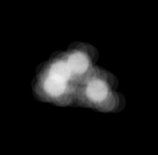
\includegraphics[width=5cm]{alphablending.PNG}
  \end{center}
  \caption{\alpha 値による半透明処理}
  \label{fig:alphanum}
\end{figure}
(openGL入門テクスチャマッピング床井浩平p21)
画像データの形式は，主に「光の3原色」(赤，緑，青)の3つの成分すなわち「RGB形式」で表している．しかしopenGLが内部で色を処理するときは，「RGBA」という4つの成分を取り扱う．この4つ目の成分である"A"は「アルファ値」とよばれ，一般に「不透明度」として扱われる．α=0なら透明，α=1なら不透明である．このα値を用いた混合処理をアルファブレンディングという．
　openGLでは，このα値を用いて2つのオブジェクトの色をglBlendFunc()という関数を用いて表現できる．引数にGL_SRC_ALPHA，ONE_MINUS_SRC_ALPHAを持つことで混合係数を決め，半透明物体の色を表示するときにα値を用いて背後の色と混合することで，半透明物体を描画することが可能である．(関数の説明)

\subsection{アルファブレンディンド}
(谷川さん論文参考)
　　フレームバッファ中に保存されている各画素の色と次に描写するポリゴンの色を混合する機能である．混合させることで半透明な表現が可能である．　
　アルファブレンディングとは，2つの画像の色を係数アルファ値により合成することである．アルファ値は画像とは独立して指定することが出来ることもあるが，画像の各画素にアルファ値を持たせてそれを利用することによって画素ごとの半透明処理も行うことが可能な機能である．
 OpenGLでは，glBlendFunc()という関数を用いてアルファブレンディングの処理を行うことが可能である．2つ以上の画素が重なっている場合，背後の色とひとつずつ半透明合成の処理をしながら描いていく．その場合，内部処理は以下の数式になる．
　 n枚の画像が重なっているとすると，その画素値Iは，背景の色をInとすると，次式で表される．
\begin{equation}
   I = \alpha_{0}I_{0}+\alpha_{1}I_{1}(1-\alpha_{0})+\alpha_{2}I_{2}(1-\alpha_{0})(1-\alpha_{1})+\cdotst+(1-\alpha_{0})(1-\alpha_{1})\cdots(1-\alpha_{n-1})\alpha_{0}I_{0}+(1-\alpha_{0}){\alpha_{1}I_{1}+(1-\alpha_{2}I_{2}+\cdot\cdot\cdot+(1-\alpha_{n-1})I_{n})} \label{exp:alpha1}
\end{equation}
式\ref{exp:alpha1}を漸化式に表現すると，式\ref{exp:alpha2}となる．
\begin{equation}
 I_{n} = \alpha_{n}I_{n}+(1-\alpha_{n})I_{n+1}\label{exp:alpha2}
\end{equation}
視点から遠い場所のポリゴンから順に，アルファブレンディングによって背後の色と混合を行う．全体のポリゴンを混合しながら重ねていくことで，雲の半透明な表現を実現する．

\subsection{ソーティング}
本研究は最終的な描画にはアルファブレンディング処理(半透明)を用いる．このアルファブレンディング処理を行うためにはソート処理が必要である．理由はzバッファとアルファブレンディングの関係で，ソートを行わないとうまく描画できないためである．(C++日本語リファレンス　std::sort　参考)
(←詳しくかけたらこのページ見て書く)

(あるごりずむ　広瀬貞樹　著　p33より引用)
ソーティングとは(sorting:整列)とは，データを”ある順序”に従って並べ替える処理のことである．例えば，氏名を”あいうえお順”に並べ替えるとか，”成績の良い順”に並べ替える等，我々の身近にしばしば見受けられる処理である．一般のプログラムは言うに及ばず，データベース等の大量うデータを高速に処理するプログラムにおいては欠かせない，もっとも基本的で重要な処理の1つである．したがって，これまで数多くのソーティングアルゴリズムが提案されそれらの特徴や性質が調べられている．\\
　代表的なソーティングアルゴリズムは選択法，挿入法，バブルソートがよく知られている．これらのアルゴリズムは全データの中から最小の値を見つけ，その最小の値を最初の値と入れ替えるなどの処理をしなければならない．しかし本研究ではC++の標準テンプレートライブラリであるsort()関数を使用しソート処理を容易に行った．\\
sort()関数\\
  template <class RandomAccessIterator>\\
  void sort(RandomAccessIterator first, RandomAccessIterator last);\\
  template <class RandomAccessIterator, class Compare>\\
  void sort(RandomAccessIterator first, RandomAccessIterator last, Compare comp);\\
　この関数は範囲を並び替えるものである．RandomAccessIteratorはValueSwappableの要求を満たしている必要があり，*first の型は MoveConstructible と MoveAssignable の要件を満たしている必要がある．要件を満たすことで[first,last）の範囲をソートできる．計算量は平均約NlogNである．\\
本研究では視点がz軸の負の方向を向いているため，点のz座標値が小さいものほど遠方にあることになる．そのためここでは点は昇順に並ぶように定義する．また，構造体を用いて粒子を発生させているため，構造体内で比較演算子を定義する必要がある．

\section{レンダリング谷川さん引用}
レンダリングとは，モデリングによってつくられたデータを可視化できるようにする作業のことである．一般的な工程は，移動，回転，および投影の座標変換をし，線画として表示する場合には陰線消去を，陰影画像なら陰面消去を施し，最後にシェーディングを行ってディスプレイにラスタライズ←？する．
　3次元物体を表示するレンダリングの基本となる陰線，陰面消去法には，奥行きソート法や，Zバッファ法，スキャンライン法，レイトシーイング法などの手法がある．これらの方法は，明確な境界面を持つ物体，とくに多面体を処理対象とした場合に有効である．しかし，濃度分布のような明確な境界面の存在しない物体を表すボリュームデータを取り扱う方が自然な場合も多い．この場合，ボリュームデータを直接レンダリングする方法としてボリュームレンダリングがある．

\subsection{ボリュームレンダリング谷川さん引用}
　ボリュームレンダリングは，3次元空間に分布する物質量(ボリュームデータ)からポリゴンデータを生成せずに，直接レンダリングして画像を生成する手法の総称である．医用画像や炎，霧，雲など，形がはっきりしないものを，ボリュームデータとして扱う場合に有効なのが，このボリュームレンダリングである．ここでのボリュームデータとは，ボクセルデータのことであり，主に3次元配列にスカラー値やベクタ値(例:X線吸収量，測定値，温度などの物理量，速度，濃度分布)を格納したものの総称のことを言う．
　ボリュームレンダリングでは，ボリュームデータを各視に沿って，一定間隔でサンプリングし，その値を加算していくことでその画像の色を決定する．また，核ボクセルに不透明度アルファ値(0が透明，1が不透明)を与えることで，ボリュームデータの内部を半透明表示にして可視化することが出来る．不透明度アルファはボクセル値そのものを用いることもあるが，隣接するボクセルのあたりからの勾配に基づいてアルファ値を決定する方法もある．


\section{粒子の運動モデル}
 本研究では通常の雲を表現する方法で用いられるパラメータ，大気の浮力，温度，圧力などは使用しない．触れる、乗れるような雲のようなものを表現するためには粒子間をなんらかの力でつなぐ必要がある．そこで，粒子と粒子を結ぶ線分をばねと考え，粒子に力が加わるとばねが伸び，触れる，乗れるといった挙動を表現する．またここでは加えられた力を押し戻すという力は考慮しないので，物体が触れると雲のようなものの力が加わった部分がへこみ，物体が沈むといった表現となる．\\
 また，ばねの質点モデルは近傍の点が分かっているので点と点の間に加わる力を簡単に計算できるが，本研究は粒子をランダムに発生しさせているため一定の範囲内にある粒子間のみの力を計算する．そのため近傍の粒子を探索する必要がある．これは物体が触れた粒子から一定の範囲内の粒子を探索しそれらの力を計算することで解決する．\\
　
\subsection{ばねの質点モデル}
　粒子を「質点」とし，粒子と粒子を結ぶ線分を「ばね」と考える．\\
 文献[1]ページ4.5課題3.4によると→（ここから床井先生の資料）\\
ばねにちからをかけない状態の長さを，ばねの自然長と呼ぶ．この長さをl_{0}とする．ばねの強さは，ばね定数で決まる．これをkとする．すべての質点（粒子）の質量はmとする．ばね両端の質点の位置をそれぞれp_{0},p_{1}とすると，ばねの長さLが次式で求めることが出来る．[1]
\begin{equation}
  L = |p_{1}-p_{0}| \label{exp:sample}
\end{equation}

\begin{figure} [htbp]
  \begin{center}
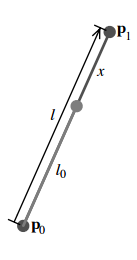
\includegraphics[height=5cm]{spring.PNG}
  \end{center}
  \label{fig:spring}
\end{figure}

ばねの力f_{s}は，ばねの伸び量をx=L-l_{0}とすると，フックの法則により，次式で求めることが出来る．
\begin{equation}
  f_{s} = -kx \label{exp:sample}
\end{equation}
この力が，ばねの伸び縮みする方向eに加わる．ばねの一方の端p_{0}を固定し，もう一方の端p_{1}を動かしたとすれば，ばねが伸び縮みする方向eは次式で求めることが出来る．
\begin{equation}
  e = (p_{1} - p_{0}) / L \label{exp:sample}
\end{equation}
したがって，p_{1}の質点に加わる力のベクトルfは次式で得られる．
\begin{equation}
  f = f_{s}e \label{exp:sample}
\end{equation}
このとき，この力を受けるp_{1}の質点の加速度aは，その質量をmとして，運動方程式f = maより次式で求めることが出来る．
\begin{equation}
 　a = \frac{f}{m} \label{exp:sample}
\end{equation}
この加速度で働く質点の時間間隔dt秒後の速度vは，初速度をv1とすると，次式で得られる．
\begin{equation}
  v = v_{1} + ad_{t} \label{exp:sample}
\end{equation}
この質点の経過時間d_{t}秒後の位置pは，現在の位置p_{1}から次の位置に移動する．
\begin{equation}
  p  = p_{1} + vd_{t} \label{exp:sample}
\end{equation}
得られたこれらの速度や位置で質点が動くアニメーションにするため，初速度や現在の位置を更新する．
\begin{equation}
  p_{1} ← p
  v_{1} ← v 
\end{equation}
 また，ばねの各点に加わる力を求め，すべての点が動くようにする．そのために，i番目の点に加わる力は，i番目とi-1番目の点を結ぶ点と，i番目とi+1番目の点を結ぶばねの力を合計したものである．\\

（図予定）
←(ここまで床井先生の資料)

 これらの式をもとにし，p_{0}，p_{1}を結ぶ線分について力を計算し，これによりp_{1}の位置を更新し質点が動くアニメーションを作成する．

%
%\subsection{ダンパモデル}
%  (ここから床井先生の資料)→文献[1]6ページ課題6より現実のばねは，無限に動き続けることはない．そこで，このばねをばねとばねの動きを抑えるダンパで構成されていると考える．\\
% このダンパによる抵抗力は，質点間の相対速度に比例するものとする．p_{0}の質点速度をv_{0}，p_{1}の質点速度をv_{1}，ダンパの減衰係数をc>0とすると，ばねの力ｆは次のようになる．
%\begin{equation}
%  f = ma + c(v_{1}-v_{0}) \label{exp:sample}
%\end{equation}
%したがってp1の質点の加速度aは，次式で求められる．
%\begin{equation}
%  a =  \frac{(f - c(v_{1}-v_{0}))}{m} \label{exp:sample}
%\end{equation}
%これにより2点間にかかる力は，その2点を結ぶばねによる力fに対して，f - c(v_{1}-v_{0})となる．『(見直す必要あり)そこで，本研究では手動で減衰係数を調整し，ダンパによる効果を追加する．』

\subsection{修正オイラー法}
 (ほぼ床井先生の資料引用→資料7-微分方程式の数値解放より)
 微分方程式の数値解放には自然現象など，様々な現象をモデル化するために使われる．例えば，投げたボールの軌道が放物線になるといった物理現象は関数として記述できる．しかし，プログラム上で実装しようとしている現象は未知の関数の場合もある．そのような場合に未知の関数とその微分の関係によって現象を記述しようとするのが微分方程式である．
 微分方程式を用いると，未知の関数，すなわち関数の形が決められない，パラメータを単純なグラフに出来ない現象であっても，現象の過去から積み重なった「今」の状態からこれからその現象がどのような動きをするのかという「性質」は決めることが出来る．
 例えば，現在時刻 t における位置 p(t) と、その時刻における速度 v(t)が分かっているとする．現在時刻から \Delta t 後の位置 p(t + \Delta t) は，速度 v(t) と時間 \Delta tを掛けたものを現在位置 p(t) に足して得られます。しかし，時刻 t から t + \Delta t の間に速度v(t) は変化するので，これは \Delta t を詳細にし，速度 v(t) に微小時間 d_{t} を掛けたものを時刻 t から t + \Delta t の間で累積，すなわち積分する必要がある．
\begin{equation}
  p(t + \Delta t) = p(t) + \int^{t+\Delta t}_{t} v(t)d_{t} \label{exp:sample}
\end{equation}

\begin{figure} [htbp]
  \begin{center}
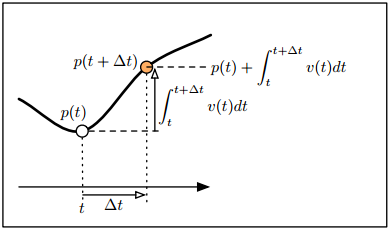
\includegraphics[width=5cm]{euler1.PNG}
  \end{center}
  \label{fig:euler1}
\end{figure}

 しかし，このv(t)の積分は風が吹く，急ブレーキをかけるなど様々な条件によって変化する．単純な積分では正確な値が分からないので，値を予測する必要がある．ここでは時刻tにおける速度v(t)を用いて\Delta t後の位置p(t+\Delta t)の値を予測する．\\
微分方程式においてこの値を予測する方法がいくつかある．オイラー法，修正オイラー法，改良オイラー法などが用いられている．\\
オイラー法とは，場合時刻tからt+\Delta tの間に速度v(t)が変化しないと仮定し，次のような予測をする．
\begin{equation}
  p(t + \Delta t) = p(t) + v(t)\Delta t \label{exp:sample}
\end{equation}
オイラー法は\Delta tが小さいほど予測の精度が向上するが，それでもこの方法による予測の誤差は大きいのでこの予測を繰り返すと誤差が累積されていく．

\begin{figure} [htbp]
  \begin{center}
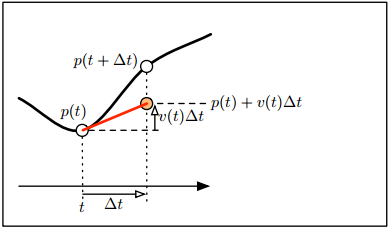
\includegraphics[width=5cm]{euler2.PNG}
  \end{center}
  \label{fig:euler2}
\end{figure}

このオイラー法の欠点を修正した方法が修正オイラー法や改良オイラー法である．修正オイラー法や改良オイラー法はt+\Delta tにおける速度v(t+\Delta t)を自力で求める必要がある．この速度は加速度を積分して求めることが出来る．また時刻tにおける加速度a(t)はその時にかかっている力などから求めることが出来る．これらから次式によりt+\Delta tにおける速度を予測する．
\begin{equation}
  v(t + \Delta t) = v(t) + a(t)\Delta t \label{exp:sample}
\end{equation}
この速度の求め方はオイラー法と同じ方法を用いることが出来る．これをv(t)に加えることでv(t+\Delta t)を求めることが出来る．このt秒後とt+\Delta t秒後の速度の平均を使って予測する方法を修正オイラー法という．
\begin{equation} 
  p(t + \Delta t) = p(t) + \frac{1}{2}(v(t)+v(t+\Delta t))\Delta t \label{exp:sample}
\end{equation}
修正オイラー法はある程度正確であり，とくに位置の二次微分である加速度を使って予測する場合は安定して答えが得られる．\\

\begin{figure} [htbp]
  \begin{center}
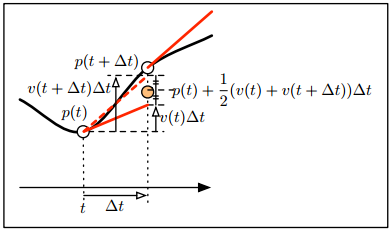
\includegraphics[width=5cm]{euler3.PNG}
  \end{center}
  \label{fig:euler3}
\end{figure}

また，時刻tからt+\Delta tの区間の中央における速度v(t + \frac{\Delta t}{2})を使用して予測する方法もある．これが改良オイラー法である．改良オイラー法を使う場合もまずオイラー法を使ってt+\Delta t秒後の位置p(t+\Delta t)とt + \frac{\Delta t}{2}秒後の速度v(t + \frac{\Delta t}{2})を予測する．
\begin{equation}
  v(t + \frac{1}{2}\Delta t) = v(t) + a(t)\frac{1}{2}\Delta t \label{exp:sample}
\end{equation}
\begin{equation}
  p(t + \Delta t) = p(t) + v(t+\frac{1}{2}\Delta t)\Delta t \label{exp:sample}
\end{equation}

\begin{figure} [htbp]
  \begin{center}
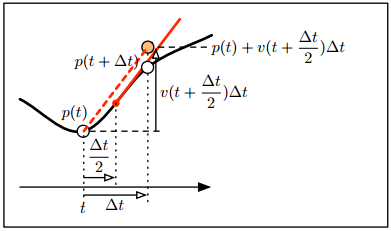
\includegraphics[width=5cm]{euler4.PNG}
  \end{center}
  \label{fig:euler4}
\end{figure}

この方法は予測に使う区間\frac{\Deltat}{2}がオイラー法の半分なので，この方法もオイラー法より正確な値を求められる．\\
修正オイラー法や改良オイラー法は，二次のルンゲクッタ法とも呼ばれる．より高い精度の予測を行う場合は，四次のルンゲクッタ法や，それをさらに改良したルンゲクッタギル法が用いられることがある．本研究では修正オイラー法を用いた予測を行っている．

\subsection{粒子探索}
 ばねの質点モデルはpが3要素の配列m×n個からなる3次元配列などと決まっているため，縦，横，斜め方向のばねの力を求めると良いことが分かっている．しかし本研究では，粒子はランダムで発生するため，1つの粒子に繋がっているどのばねの力を計算するのか明らかになっていない．また，1つの粒子はそれ自身を除くすべての粒子と繋げられるため，それらのばねの力をすべて計算することは膨大な時間がかかってしまう．この問題を解決するために，粒子探索という方法を用いる．\\
　本研究では力が加わった点から一定の範囲内にある粒子間のばねの力を計算するために粒子探索を用いる．

　範囲は任意に設定する
　また，ここでは円を使って粒子探索を行う．

\subsection{力が及ぶ範囲設定}





粒子は主な円形に発生いさせた粒子の塊を数個用い、その塊を中心に周りの粒子を発生させ形を形成する．まずはじめに粒子の塊の中心部分をメルセンヌツイスター法による乱数を用い，一様実数分布で粒子を発生させる．

\section{結果}


\section{今後の課題}
雲の形は多岐にわたり，人によって雲の形はこうあるべきという概念が異なり，映像では場面ごとに使いたい雲の形が異なる．なので，ユーザの作りたい雲の形を作れるよう，パラメーターを調整すると雲の形が容易に変更できるソフトウェアを開発することが必要となってくる．また，ばねの力もパラメータを変更することで容易に変更可能なソフトウェアを開発し，ユーザが作りたい雲の形，挙動を作成できるソフトウェアを開発を行う．また，本研究では実現できなかった力が加えられた場合に雲の粒子が飛び散るという挙動を実現するため，よりリアルな雲の見た目を作るために粒子法を実装していく．


\chapter{参考文献}
[1]メディアデザインセミナー資料 ばね質点モデル 床井浩平

記述すべき項目は，
\begin{itemize}
  \item タイトル
  \item 坂口美優
  \item 学士(4年)
  \item デザイン情報学科
  \item 60195023
  \item 卒業年度
  \item 論文提出日
\end{itemize}
である．．


\chapter{図，表，数式}\label{chap:fig-tab-exp}

論文では，図，表，数式などを効果的に使用する．

\section{図}

{\tt figure}環境を利用することによって図にキャプション
(\verb|\caption|)を付けることができる．図に付けられたキャプションは
\verb|\listoffigures|によって図目次として出力される．図には章ごとに通
し番号が付けられ，キャプションに\verb|\label|を設定しておくと，
``図\ref{fig:sample}''のように\verb|\ref|によって図を番号で参照するこ
とができる．図\ref{fig:sample}に{\tt figure}環境を用いた記述例を示す．











\section{表}

{\tt table}環境を利用することによって図と同じように，キャプションをつ
けたり，ラベルにより参照したりすることができる．また
\verb|\listoftables|によって表目次として出力される．
表\ref{tab:sample}に{\tt table}環境で作成した表を示す．

\begin{table}
  \caption{表の例}
  \label{tab:sample}
  \begin{center}
    \begin{tabular}{|c|c|c|}
      \hline
      8 & 3 & 4\\
      \hline
      1 & 5 & 9 \\
      \hline
      6 & 7 & 2 \\
      \hline
    \end{tabular}
  \end{center}
\end{table}

\section{数式}

\TeX では数式のための機能が豊富である．
{\tt equation}環境などを利用することによって数式に番号を付けることがで
きる．図や表と同じくラベルを付けておけば，``式\ref{exp:sample}''のよう
に数式を番号で参照することができる．

\begin{equation}
  y = ax^2 + bx + c \label{exp:sample}
\end{equation}

\chapter{参考文献}

文献を参照する場合には，論文の最後に参考文献として列挙するとともに，
\verb|\cite|を使って，例えば，
\begin{quote}
  文献\cite{latex}によれば…
\end{quote}
や，
\begin{quote}
  …である\cite{latex2e}．
\end{quote}
のように参照する．

文献の列挙には，{\tt thebibliography}環境などを用いる\footnote{使い方
は，この資料のソースを参照．}．

%%%%%%%%%%%%%%%%%%%%%%%%%%%%%%%%%%%%%%%%%%%%%%%%%%%%%%%%%%%%%%%%%%%%%%%%

%%
%% 謝辞
%%
%% \begin{acknowledgements}
%% 感謝します．
%% \end{acknowledgements}

%%%%%%%%%%%%%%%%%%%%%%%%%%%%%%%%%%%%%%%%%%%%%%%%%%%%%%%%%%%%%%%%%%%%%%%%

%%
%% 参考文献
%%
\begin{thebibliography}{99}
\bibitem{wusethesis}
    和歌山大学システム工学部卒業論文/大学院システム工学研究科修士論文用スタイルファイル，
    ``{\tt http://www.wakayama-u.ac.jp/\symbol{"7E}fukuyasu/gres/}''．
\bibitem{latex}
    奥村晴彦，\LaTeX 入門---美文書作成のポイント---，技術評論社，1993．
\bibitem{latex2e}
    奥村晴彦，黒木裕介，[改定第6版] \LaTeXe~美文書作成入門，技術評論社，2013．
\bibitem{texbasic}
    OfficeMASA，神代英俊，長島秀行 著，\TeX の基礎，
    ソフトバンクパブリッシング，2002．
\bibitem{latexcomp}
    M. Goossens, F. Mittelbach, A. Samarin 共著，
    アスキー書籍編集部 監訳，The \LaTeX コンパニオン，アスキー出版局，1998．
\end{thebibliography}

%%%%%%%%%%%%%%%%%%%%%%%%%%%%%%%%%%%%%%%%%%%%%%%%%%%%%%%%%%%%%%%%%%%%%%%%

%%
%% 付録
%%
% \appendix
% 
% \chapter{サンプルプログラム}
% 
% プログラムリストや実行結果など，本論を補足する上で必要と思われるものが
% あれば付録として付ける．
% 
% {
% \footnotesize
% \begin{verbatim}
% #include <stdio.h>
% int main(void)
% {
%     printf("Hello, World!\n");
%     return 0;
% }
% \end{verbatim}
% }

%%%%%%%%%%%%%%%%%%%%%%%%%%%%%%%%%%%%%%%%%%%%%%%%%%%%%%%%%%%%%%%%%%%%%%%%

\end{document}
